Dieses Kapitel stellt eine Zusammenfassung der wichtigsten Ergebnisse dieser Arbeit auf, die zur Beantwortung der Thesen führen. Es werden zusammenfassend die Grenzen und Einschränkungen geklärt, zu denen die Evaluation durchgeführt wurde. Des Weiteren werden Impulse für weitere Forschungen diskutiert. Das Kapitel endet mit einer praktischen Anwendung, bei der die Ergebnisse dieser Arbeit angewandt werden können.

%Vergleich Stand der Forschung: fehlt noch, muss in Thesen einfließen

\section{Bewertung der Zielsetzung und Thesen}
% 3. These: Optimierung ohne Modellanpassung, nur Prompt Engineering
Die Erkenntnisse aus den Experimenten dieser Arbeit bestätigen die aufgestellte dritte These (T3) aus Kapitel \ref{sec:goals_of_the_work}. Eine Optimierung der Eingabeaufforderungen für die Webanwendungsentwicklung lässt sich ohne Änderung der Modellparameter erreichen und bewirken, für einige Modelle eine signifikante Verbesserung der Ergebnisse. Die Modelle wurden bereits mit Programmiersprachen, die für Webanwendungsentwicklung essenziell sind trainiert, wie beispielsweise mit PHP, diese Daten sind in Form von Programmcode und sind von den Modellen abrufbar. Entscheidend hierbei ist die Art und Weise wie die Gestaltung der Eingabeaufforderungen umgesetzt wird. Diese Optimierung erfolgt durch das \texttt{DSPy} Framework für viele Modelle automatisiert.\vspace{0.2cm}

% Hat nicht funktioniert.
Dennoch hat das \texttt{DSPy} Framework, auf einige Modelle einen negativen Effekt. Der generierte Code, dieser Modelle schnitt in der Evaluation mit den HumanEval-XL Proben schlechter ab. Der Grund konnte zurzeit nicht geklärt werden. Eine Annahme ist, dass der deklarative Ansatz von \texttt{DSPy} mit den komplexeren Datenstrukturen und Modulketten die LLMs zu inkonsistenten Antworten leitet. In diesen Fällen sollte weitere Frameworks, wie beispielsweise \textit{AdalFlow} oder \textit{LamaIndex} für die Optimierung in Betracht gezogen werden.\vspace{0.2cm}

% Es gibt Fehler bei der Verwendung von DSPy.
Die Tests haben weiterhin gezeigt, dass einige Modelle nicht mit dem \texttt{DSPy} Framework zusammenarbeiten. Auch hier konnte nicht abschließend geklärt werden, ob die Fehlerquelle bei der eingesetzten Hardware zu suchen ist oder ob das Framework selbst Probleme mit den Antworten dieser Modelle hat. Bei Modellen, die dieses Verhalten zeigen, sollte geprüft werden, ob auch hier die Wahl auf ein anderes Framework fallen kann.\vspace{0.2cm}

Gerade mit der Arbeit von Closed-Source-Modellen, bei der die Modelle gar nicht oder nur sehr bedingt angepasst werden können, sind die Optimierungen der Eingabeaufforderungen essenziell. Hierbei kann ein Framework, wie das \texttt{DSPy} eine hilfreiche Unterstützung bieten.\vspace{0.2cm}

% 2. These: Benckmarks sind ungeeignet
Alle Evaluierungen wurden mit den HumanEval-XL durchgeführt. Mit den gewonnenen Erkenntnissen aus dieser Arbeit lässt sich die zweite These (T2) nur bedingt bestätigen. Ein einzelner Benchmark hat nicht ausreichend Aussagekraft, um eine LLM hinreichend zu bewerten. Diese Benchmarks eignen sich um einen ersten Eindruck von den Modellen zu erhalten. Hierbei können erste Eindrücke über deren Stärken und Schwächen gesammelt werden. Wie auch in \cite{zhang-2024} wird die Auffassung vertreten, dass diese Probe grundlegende Codeproblematiken testen, die nicht mit den realen Anforderungen von Entwicklern übereinstimmen. Diese Aussagen deuten darauf hin, dass Programmierer andere Anforderungen an LLMs stellen, die zurzeit mit Benchmarks, nur in engen Grenzen abgedeckt werden können. Zu beachten ist weiterhin, dass die Benchmarks nicht frei von Fehlern sind, die eine verzerrtes Bild der LLM erzeugen können. Entwickler würden die Fehleingaben in den Eingabeaufforderungen berichtigen und einen erneuten Versuch unternehmen, Code generieren zu lassen.\vspace{0.2cm}

%benchmark prüfen auf fehler
Die menschliche Intelligenz ist in der Lage aus generiertem Code und eigenem Wissen, die Programmteile herauszufiltern welche zur Lösung eines Problems beitragen. Entwickler stellen meist sehr komplexe Anforderungen, um die ihnen gestellten Probleme zu lösen. Diese Komplexität wird durch die Benchmarks nicht abgedeckt.\vspace{0.2cm}

% 1. These: LLMs effizientere Webanwendungsentwicklung. Wichtig ist die Evaluierung
In den letzten Jahren hat generative KI auch die Arbeit der Entwickler stark beeinflusst. So ist in \cite{focus-online-2025} die Rede von einem Programmierer, der seine Aufgabe abbrach, Zitat: \glqq \textit{weil er keinen Zugang zu seinem virtuellen Assistenten hatte. ''Ich kann einfach nicht mehr ohne die Hilfe der KI programmieren''}\grqq \ so der Entwickler. In \cite{company_gartner_2024}, einem Artikel von Gartner, wird behauptet das bis zum Jahr 2027, 80\% der Ingenieure eine Weiterbildung für generative KI benötigen. Dies hebt ebenfalls den Trend der nächsten Jahre hervor, das generative KI die Softwareentwicklung maßgeblich beeinflussen wird. Zurzeit sollten Entwickler sich aber nicht voll auf die Ausgaben der LLMs verlassen. Dies bestätigt auch der Onlineartikel \cite{albrecht-2023}, in diesem heißt es, Zitat: \glqq \textit{ChatGPT ... liefert Code, der zwar nicht immer direkt nutzbar ist, nach einer Überarbeitung aber schon recht überzeugend läuft.}\grqq.\vspace{0.2cm}

% Zu den Modellen.
Trotzdem wächst die Beliebtheit von KI Anwendungen bei Softwareentwicklern immer weiter und dies gilt auch für den Bereich der Webanwendungsentwicklung. Dabei nutzen viele Entwickler, KI Modellen von US amerikanischen Unternehmen wie Athropic, Google oder OpenAI die bereits sehr gut entwickelte Chatbots und APIs anbieten, welche für die Integration in Tools zur Codegenerierung eingesetzt werden können. Zurzeit hat Mistral, eine europäische KI-Entwicklungsfirma einen neuen Chatbot, mit dem Name \textit{Le Chat} herausgebracht, der als Konkurrenz zu den amerikanischen Konzernen gesehen wird. Die KI-Entwicklungsfirma \textit{Deepseek} aus China hat ein Modell entwickelt, das wie Mistral, in Konkurrenz zu den amerikanischen Modellen steht. Neben diese kommerziellen Closed-Source-Modelle gibt es eine Reihe von Open-Source-Modellen und einige Entwicklungsfirmen wie Mistral oder Deepseek bieten neben den kommerziellen, auch einige ihrer Modelle als Open-Source an. Diese Modelle zeigen ebenfalls hervorragende Resultate für die Generierung von Code, wie die Ergebnisse dieser Arbeit beweisen. Um so wichtiger ist es die Stärken und Schwächen der Modelle zu kennen und welche Methoden, zur effektiven Nutzung von Eingabeaufforderungen einzusetzen sind. Mit diesen Kenntnissen wird die, in der Arbeit aufgestellte dritte These (T3) bewiesen. Ki kann und wird die Webanwendungsentwicklung maßgeblich beeinflussen.\vspace{0.2cm}

Gerade die einfache und effiziente Suche mithilfe der LLMs bring einen zeitlichen Vorteil, dessen Ergebnisse bereits mit einfachen Tests überprüft werden können. LLMs reduzieren die Suche nach geeigneten Frameworks und Technologien und liefern oft funktionsfähigen Code. Dies gilt für die Integration in \acrshort{IDE} wie auch die Nutzung eines Chatbots.

\section{Grenzen und Einschränkungen}
%Kleine Beteiligung der Closed-Source-Modelle aufgrund der Kosten.
Die in dieser Arbeit evaluierten und optimierten Modelle, waren hauptsächlich Open-Source-Modelle. Alle diese Modelle wurden von der Plattform Ollama bereitgestellt. Zwei Ausnahmen gab es bei der Evaluierung, hierbei handelt es sich um \textit{Gemini 1.5} von Google und \textit{ChatGPT 4} von OpenAI.\vspace{0.2cm}

%Benchmark nur den HumanEval-XL, mit 80 Proben.
Für die Evaluierung der Modelle ist nur der \textit{HumanEval-XL} angewandt worden. Die meisten Benchmarks prüfen LLMs mit Python oder Java Proben. Eine Evaluierung mit spezifischen Sprachen für Webanwendungsentwicklung wie PHP, bieten nur wenige Benchmarks, darunter der \textit{HumanEval-XL}.\vspace{0.2cm}

%Nur langchain und DPSy
Die Auswahl der getesteten Frameworks, welche die Kommunikation zu den LLMs und somit zum Ollama-Server herstellten, waren begrenzt auf \texttt{langchain} und \texttt{DSPy}.\vspace{0.2cm}

\section{Impulse für zukünftige Forschungen}
%Ein interessantes Feld für die Forschung ist die Nutzung generativer KI und welche Auswirkungen dies auf das menschliche Denken und Handeln hat. In der Studie \cite{chiriatti-2024} wird von einem System 0 gesprochen, welches neben den bekannten 
%\begin{enumerate}
%	\item System 1: schnelles,intuitives und automatisches Denken
%	\item System 2: langsameres, analytisches und reflektierteres Denken
%\end{enumerate}

%eingeführt wird. Hierbei handelt es sich um ein Denken, welches die KI für den Menschen übernimmt. Entscheidungen und Daten werden durch die KI übernommen. Ein externes System, ähnlich wie eine USB-Festplatte eines PCs.\vspace{0.2cm}
% Immer neue Modelle
Die KI-Entwicklungsfirmen bringen immer neue Modelle auf dem Markt, die schon mit einer sehr kleinen Anzahl vom Parametern gute Ergebnisse liefern. Hier könnte eine Studie zeigen, ob \textit{Small Language Models} (SLM) mit den \textit{Large Language Models} (LLM), im Bereich der Webanwendungsentwicklung konkurrieren können. Ein Beispiel für ein SML ist das Modelle \textit{Phi} von Mirosoft, welches beispielsweise unter \cite{phi2_huggingface_2024} heruntergeladen werden kann. Wird ein kleines Modell für die Codegenerierung eingesetzt und dahin gehend optimiert, ist eine große Parameteranzahl nicht erforderlich. Es existieren bereits einige Studien zu diesem Thema. Beispielsweise wird in \cite{hu-2024} eine allgemeine Verbesserung des Benutzererlebnisses untersucht und in \cite{irugalbandara-2023} wird eine Reduzierung der Kosten in Produktionsumgebungen vorgestellt.\vspace{0.2cm}
%Inwieweit können auch \textit{Small Language Models} für Programmieraufgaben eingesetzt werden. Könnte der enorme Energiebedarf und Ressourcen der LLMs durch SLMs ersetzt werden? Siehe \href{https://medium.com/@nageshmashette32/small-language-models-slms-305597c9edf2}{Small Language Models (SLMs)} oder \href{https://medium.com/version-1/small-but-powerful-a-deep-dive-into-small-language-models-slms-b793bdb002f2}{Small but Powerful: A Deep Dive into Small Language Models (SLMs)}. Eine weitere Forschung kann die Evaluation sein, ob Finetuned SLMs, wie Phi-2, Google Gemini Nano oder Metas Llama-2-13b bessere Ergebnisse liefern, als die LLMs.\vspace{0.2cm}

% Andere Benchmakrs eigene entwickeln.
Des Weiteren sollte Unternehmen oder Entwickler weitere Benchmarks in Betracht ziehen und die Brauchbarkeit von LLMs für die Webanwendungsentwicklung evaluieren. Interessant wäre die Prüfung, ob die Verwendung mehrerer Benchmarks zu einer besseren Bewertung der LLMs führt.\vspace{0.2cm}

Da die meisten Benchmarks auf statische Analysen ausgelegt sind und die LLMs nur bedingtes oder klein deterministisches Verhalten zeigen, kann eine weitere Forschung dahin gehen, einen Benchmark zu erstellen, der auf die dynamischen Antworten der LLMs besser eingehen könnte. Speziell für die PHP-Entwicklung wäre eine Untersuchung interessant, bei der die Evaluierung mit externer Tool wie \textit{SonarQube}, \textit{PHPBench}, \textit{PHPUnit} oder \textit{PHPMetrics} durchgeführt und dadurch eine verbesserte Bewertung der LLMs erreicht wird. Analog kann so ein Benchmark auf andere relevante Programmiersprachen der Webentwicklung ausgeweitet werden, wie beispielsweise JavaScript, Java und Ruby.\vspace{0.2cm}

Weil LLMs kein deterministisches Verhalten zeigen, könnte die Auswertung der generierten Codes nicht auch von einer anderen LLM übernommen werden, sodass LLMs einander selbst bewerten? Bei so einem Verfahren, wären Forschungen möglich, ob auf externe Tools und statische Tests ganz verzichtet werden kann.\vspace{0.2cm}

% Einführung in Firmen und Schluung der Mitarbeiter.
Ein weiteres mögliches Themenfeld ist der Einführungsprozess von KI gestützten Softwareentwicklung für Webanwendungen unter Anwendung von Firmenrichtlinien. Der Fokus sollte hierbei auf das Auswahlverfahren der Modelle liegen mit Blick auf die möglichen Benchmarks und dem Evaluierungsverfahren. Wie lassen sich Entwickler frühzeitig in die Auswahl der Modelle einbeziehen und welche Möglichkeiten bestehen für Entwickler schon während dieses Prozesses ihre Kenntnisse im Bereich von generativer KI zu erweitern oder vertiefen, sodass effektives Entwickeln von Anfang an erfolgen kann?\vspace{0.2cm}
%\begin{tcolorbox}[
%	enhanced,
%	breakable,
%	colback=red!5!white,
%	colframe=red!75!black!50,
%	title= Mein roter Faden: noch was zum Testen
%	]
%	Ein Tool zur Orchestrierung von Multi-Agenten-Systemen \href{https://community.openai.com/t/introducing-swarm-js-node-js-implementation-of-openai-swarm/977510}{OpenAI Swarm}, gefunden auf \href{https://karrierewelt.golem.de/blogs/karriere-ratgeber/bot-belegschaft-mit-entlastungspotenzial-ki-agenten-fur-den-arbeitsalltag-in-der-testphase-1}{Golem | Karrierrewelt}.
%\end{tcolorbox}

\section{Praktische Anwendung}
%Praktische Anwendung: Eine Diskussion der möglichen Anwendungen der Ergebnisse. In welchen Unternehmen und welche realen Anwendungen können die Ergebnisse eingesetzt werden.
% Konkreter Fall
In der kommenden Zeit wird die Entwicklung der LLM weiter voranschreiten und dies wird zu weiteren Verbesserungen bei den Ausgaben der LLMs führen, was langfristig zu noch effizienteren Entwickeln führt. Dennoch sollte der Focus auf eine einheitliche Vorgehensweise liegen. Somit werden nicht nur gleiche Standards beim Code geschaffen, zudem wird ein einheitliches Know-How der Mitarbeiter realisiert. Dies wird langfristig dazu führen, dass die Entwicklung von Webanwendungen mithilfe generativer KI, die Arbeit der Entwickler effizienter gestaltet und sich somit auf die Kosten und Ressourcen der Unternehmen auswirkt. Was sich positiv auf die Wettbewerbsfähigkeit der Softwareunternehmen auswirken kann.\vspace{0.2cm}

% Nutzen/Vorteil
Die Auswahl der Anbieter wird, durch deren ständig wachsender Anzahl der LLMs immer schwieriger. Die in dieser Arbeit vorgestellten Ergebnisse der evaluierten Modelle, können Unternehmen nutzen, um einen Einstieg in das Thema zubekommen und schlägt Modelle vor, welche sich für die Generierung von Programmcode in der Webanwendungsentwicklung eigenen. Des Weiteren unterstützt diese Arbeit die Unternehmen den bei ersten Versuchen, weitere neue LLMs zu evaluieren und das optimale Modell für ihre Prozesse zu finden. Die Mehrheit der Entwickler und Unternehmen nutzen zurzeit kommerzielle Modelle großer Anbieter, da die Nutzung der Chatbots und die schnelle, unkomplizierte Verwendung der APIs mit wenig Aufwand realisierbar ist. Durch das zunehmende breite Interesse an generativer KI, wurden Möglichkeiten geschaffen Open-Source-Modelle in der eigenen Infrastruktur einzubinden und diese zu verwenden. Dies kann, wie schon zuvor besprochen zur Senkung der Kosten beitragen. Besonders die Abrechnung der Tokens ist ein interessanter Punkt, der nicht immer eindeutig nachvollziehbar ist. Der Kostenaspekt zwischen \textit{Open-Source} und \textit{Closed-Source} Modellen, wurde schon aufgegriffen, diskutiert und bringt laut \cite{irugalbandara-2023} eine große Ersparnis, was besonders für mittlere und große Unternehmen interessant werden kann. Wie in dieser Arbeit gezeigt, liefern die Open-Source-Modelle hervorragende Ergebnisse für die Aufgaben in der Webanwendungsentwicklung, die oft bessere sind, als die Ergebnisse der kommerziellen Closed-Source-Modelle.\vspace{0.2cm}

% Implementierung
Unabhängig von der Auswahl des Modells sollten Unternehmen für die Entwickler einheitliche Schnittstellen zu den Modellen bereitstellen. Zum Einem können die Eingabeaufforderungen, wie in dieser Arbeit beschrieben, mittels verschiedener Frameworks oder anderer Methoden angepasst werden. Zum anderen können die abgesetzten Prompts verwendet finden, um beispielsweise Modelle weiter, durch \glqq Fine-Tuning\grqq \ zu optimieren. Eine weitere Möglichkeit besteht darin die Prompts auszuwerten und den Wissensstand der Entwickler zu prüfen und gegebenenfalls mit gezielten Schulungsmaßnahmen das Entwicklungsteam zu fördern.\vspace{0.2cm}

Ein weiterer Vorteil dieser Methode ist, dass die Möglichkeit besteht Prompts mit verschiedenen Metadaten anzureichern und Ansätze wie \textit{Personas}, \textit{Beispielen} und \textit{zusätzlichem Kontext} umgesetzt werden können. Vorstellbar wäre auch die Integration eines RAG, welches auf Daten der eigenen Entwickler und bereits umgesetzter Softwarelösungen zurückgreifen kann.\vspace{0.2cm}

% Example
Die Abbildung \ref{img:example_firm_integration} zeigt das zuvor beschriebene Beispiel für die Integration einer LLM in den Prozess der Programmcodegenerierung. Die Entwickler stellen ihre Eingabeaufforderungen an den Agenten. Das erfolgt über ein Eingabeformular oder als Plug-in einer IDE. Über das Plug-in wird der generierte Code direkt in das aktuelle Projekt übernommen. Das Formular bietet die Möglichkeit weitere Fragen an die LLM stellen, die keinen Code generieren sollen. Dies könnten allgemeine Fragen zur Architektur oder Fragen zur Beurteilung von Tools beinhalten. Mit der beschriebenen Architektur, werden alle Fragen und Probleme erfasst, mit der sich die Entwickler auseinandersetzen. Diese Informationen könnten bei der Suche eines geeigneteren Benchmarks behilflich sein.\vspace{0.2cm}

% Der Agent
In einem ersten Schritt könnte der Agent als einfacher Aufruf einer LLM implementiert werden, um ihn später durch einen echten Agenten zu ersetzen. Der Agent leitet den einfachen oder optimierten Prompt an die LLM weiter, wertet die Antwort aus und sendet das Ergebnis an den Entwickler zurück. Zusätzlich werden die Prompts aufgezeichnet und in einer Datenbank gespeichert. In der Abbildung wird die Datenbank als \texttt{Logs} bezeichnet. Für die grün dargestellten Elemente, in der Abbildung \ref{img:example_firm_integration} sind in dieser Arbeit bereits Ansätze und Lösungsvorschläge vorgestellt und besprochen wurden.\vspace{0.2cm}

\begin{figure}[!ht]
	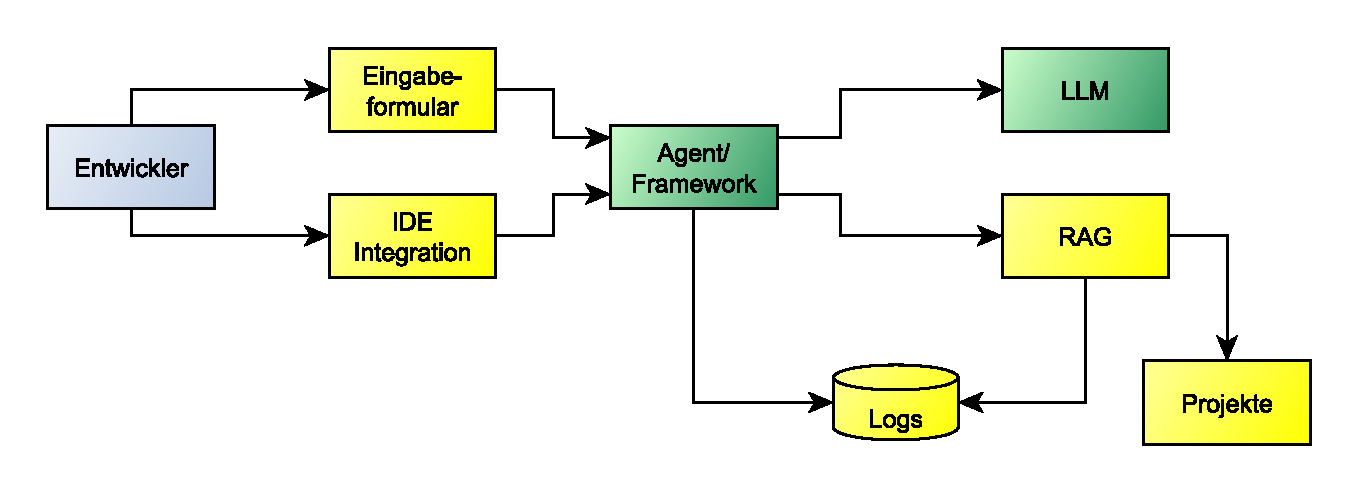
\includegraphics[width=0.9\textwidth]{content/chapter_discussion/images/anwendungsbeispiel.eps}
	\centering
	\caption{Anwendungsbeispiel für die Integration einer LLM}
	\label{img:example_firm_integration}
\end{figure}

Sobald ein Agent implementiert wurde und zum Einsatz kommt, können werte Quellen zur Informationsbeschaffung an den Agenten angeschlossen werden. Dies kann als \textit{Retrieval Augmented Generation} (\acrshort{RAG}) implementiert werden, um auf die vorhandene firmenintern Daten zuzugreifen. Diese Daten können aus bereits gestellte und bewertete Eingabeaufforderungen der Entwickler oder aus vorhandenem Codes von abgeschlossenen Projekten bestehen. Mit dem, in dieser Arbeit vorgestellten \texttt{DSPy} Framework können unter anderem Agenten und RAG implementiert werden.\vspace{0.2cm}

Abschließend wird in Abbildung \ref{img:example_chat_form} ein Beispiel für ein einfaches Chat-Formular gezeigt. Weitere Formularfelder können im Formular hinzugefügt und der LLM als zusätzliche Metadaten oder Anweisungen mitgeteilt werden.\vspace{0.2cm}

\begin{figure}[!ht]
	
\includegraphics[width=0.7\textwidth]{content/chapter_discussion/images/chatbot_form_example.eps}
	\centering
	\caption{Anwendungsbeispiel für ein Eingabeformular für Prompts}
	\label{img:example_chat_form}
\end{figure}

Allerdings kann es hierbei auch zu Problemen kommen, beispielsweise wenn Entwickler falschen Code als richtig bewerten und diese Informationen der LLM zur Verfügung gestellt werden.
%Blaupause für Prompting \href{https://piamedia.com/wp-content/uploads/2024/09/PIAM_Whitepaper_LLM-Halluzinationen_DE.pdf}{Das Geheimnis hinter LLM-Halluzinationen} [S. 16 ff.] noch testen und evaluieren.
%\href{https://arxiv.org/html/2501.16998v1}{Große Sprachmodelle zur Codegenerierung: Die Perspektive der Praktiker}
%Zur Optimierung des generierten Codes kann auch die freie Wahl der Softwarekomponenten durch die LLMs betragen. Wie in \cite{chen-2021} beschrieben können Nutzer, anstatt in Suchmaschinen beispielsweise die Vorteilen und Nachteile von \texttt{PyTorch} und \texttt{Tensorflow} zu vergleichen, kann das die LLM übernehmen und als Prompt wird nur \texttt{\# import machine learning package} angegeben.\vspace{0.2cm}
%Wie in [Quelle ist weg] beschrieben nimmt das Lesen von Programm zehn mal mehr Zeit in Anspruch, als Code zu schreiben. Diese Arbeit kann ebenfalls durch eine LLM übernommen werden.
